\documentclass[twoside]{article}
\setlength{\oddsidemargin}{0.25 in}
\setlength{\evensidemargin}{-0.25 in}
\setlength{\topmargin}{-0.6 in}
\setlength{\textwidth}{6.5 in}
\setlength{\textheight}{8.5 in}
\setlength{\headsep}{0.75 in}
\setlength{\parindent}{0 in}
\setlength{\parskip}{0.1 in}

\usepackage{graphicx}
\usepackage{url}

%
% The following commands sets up the lecnum (lecture number)
% counter and make various numbering schemes work relative
% to the lecture number.
%
\newcounter{lecnum}
\renewcommand{\thepage}{\thelecnum-\arabic{page}}
\renewcommand{\thesection}{\thelecnum.\arabic{section}}
\renewcommand{\theequation}{\thelecnum.\arabic{equation}}
\renewcommand{\thefigure}{\thelecnum.\arabic{figure}}
\renewcommand{\thetable}{\thelecnum.\arabic{table}}
\newcommand{\dnl}{\mbox{}\par}

%
% The following macro is used to generate the header.
%
\newcommand{\lecture}[4]{
  \pagestyle{myheadings}
  \thispagestyle{plain}
  \newpage
  \setcounter{lecnum}{#1}
  \setcounter{page}{1}
  \noindent
  \begin{center}
  \framebox{
     \vbox{\vspace{2mm}
   \hbox to 6.28in { {\bf COMPSCI~590S~~~Systems for Data Science
                       \hfill Fall 2017} }

      \vspace{4mm}
      \hbox to 6.28in { {\Large \hfill Lecture #1: #2  \hfill} }
      \vspace{2mm}
      \hbox to 6.28in { {\it Lecturer: #3 \hfill Scribe(s): #4} }
     \vspace{2mm}}
  }
  \end{center}
  \markboth{Lecture {#1}: #2}{Lecture {#1}: #2}
  \vspace*{4mm}
}

%
% Convention for citations is authors' initials followed by the year.
% For example, to cite a paper by Leighton and Maggs you would type
% \cite{LM89}, and to cite a paper by Strassen you would type \cite{S69}.
% (To avoid bibliography problems, for now we redefine the \cite command.)
%
\renewcommand{\cite}[1]{[#1]}

% \input{epsf}

%Use this command for a figure; it puts a figure in wherever you want it.
%usage: \fig{NUMBER}{FIGURE-SIZE}{CAPTION}{FILENAME}
\newcommand{\fig}[4]{
           \vspace{0.2 in}
           \setlength{\epsfxsize}{#2}
           \centerline{\epsfbox{#4}}
           \begin{center}
           Figure \thelecnum.#1:~#3
           \end{center}
   }

% Use these for theorems, lemmas, proofs, etc.
\newtheorem{theorem}{Theorem}[lecnum]
\newtheorem{lemma}[theorem]{Lemma}
\newtheorem{proposition}[theorem]{Proposition}
\newtheorem{claim}[theorem]{Claim}
\newtheorem{corollary}[theorem]{Corollary}
\newtheorem{definition}[theorem]{Definition}
\newenvironment{proof}{{\bf Proof:}}{\hfill\rule{2mm}{2mm}}

% Some useful equation alignment commands, borrowed from TeX
\makeatletter
\def\eqalign#1{\,\vcenter{\openup\jot\m@th
 \ialign{\strut\hfil$\displaystyle{##}$&$\displaystyle{{}##}$\hfil
     \crcr#1\crcr}}\,}
\def\eqalignno#1{\displ@y \tabskip\@centering
 \halign to\displaywidth{\hfil$\displaystyle{##}$\tabskip\z@skip
   &$\displaystyle{{}##}$\hfil\tabskip\@centering
   &\llap{$##$}\tabskip\z@skip\crcr
   #1\crcr}}
\def\leqalignno#1{\displ@y \tabskip\@centering
 \halign to\displaywidth{\hfil$\displaystyle{##}$\tabskip\z@skip
   &$\displaystyle{{}##}$\hfil\tabskip\@centering
   &\kern-\displaywidth\rlap{$##$}\tabskip\displaywidth\crcr
   #1\crcr}}
\makeatother

% **** IF YOU WANT TO DEFINE ADDITIONAL MACROS FOR YOURSELF, PUT THEM HERE:



% Some general latex examples and examples making use of the
% macros follow.
\graphicspath{ {} }

\begin{document}

%FILL IN THE RIGHT INFO.
%\lecture{**LECTURE-NUMBER**}{**DATE**}{**LECTURER**}{**SCRIBE**}
\lecture{12}{Graph Storage}{Emery Berger}{Ariel Reches, Saranya Krishnakumar}

\section{Representing Graphs}

How can we represent graphs, how do they fit into any of the previous big data storage frameworks we learned?. To work on graphs using previous data storage systems, graphs had to be represented in a matrix or list form and then worked upon.
\begin{enumerate}

\item Database systems we know :
\begin{enumerate}
\item NoSQL, Map Redpuce, Key Values
\item SQL, Reg Databases, tuples
\item OOdatabases, "objects", XML for example
\end{enumerate}

\item Representing Graphs :
\begin{enumerate}
\item Ways to represent :
\begin{enumerate}
\item Adjacency Matrix - symmetric along diagonal for undirected graph, hence only half of the matrix needs to be stored, $O(V^2)$
\item Adjacency List - vertex edge notation, $O(V + E)$ ex. 1(2,3) 4(5,6)
\item (Edge, Edge) - every edge is represented as set of vertices, $O(2E)$ ex. (1,2) (1,3) (4,5) (4,6)

\end{enumerate}
\item Degrees of Freedom :
\begin{enumerate}
\item Directed/Undirected - when connections are symmetric undirected graphs are used, when connections are asymmetric directed graphs are used for representing(Twitter relationship vs Facebook relationship)
\item Static vs Dynamic (Points on a map vs friends in a social network)
\end{enumerate}


\end{enumerate}

\end{enumerate}

\section{Sparse Graphs}
A sparse graph is one in which many pairs of vertices do not share any edges. An adjacency matrix is an inefficient way to hold sparse graphs even considering the benefit that all graph operations can be turned to matrix operations. Most of the graphs in general are sparse, ex. in social networks like Facebook, there are lesser than $N^2$ edges, not everyone is friends with everyone else. Complete graphs are unlikely in reality. Hence we need optimal way of representing sparse matrices.
\begin{enumerate}
\item Matrix representation bad for sparse data
\item Run Length encoding ex. (1, 1, 4, 1) = starting at 1,1 there are 4 1s in a row
\begin{enumerate}
\item Good for sparse matrices generally but usually doesn't work for graphs
\end{enumerate}
\item Sparse graph usually uses adjacency list $O(V + E)$ or (vertex, vertex) $O(2E)$
\end{enumerate}

\section{Map Reduce with Edge List}
Map Reduce with Edge Lists is bad for a few reasons
\begin{enumerate}
\item Too much IO (many Map steps involving disk write/ disk read)
\item Close edges likely to be widely distributed across cluster(poor locality)
\item Map Reduce completely oblivious to the graph structure
\end{enumerate}

\section{Graph Computation}
Previously all graph computations were run in one machine. But this was not efficient for processing large graphs. Hence distributing computation across many machines was introduced in Pregel. Pregel is a vertex centric model. All edges with a vertex are stored locally along with the vertex, so that no message passing is required between vertex and edge for computation, also gives fault tolerance. Pregel does not work when there are too many edges associated with a vertex (ex. Jutin Bieber and Ellen Degeneres problem).

\section{BSP + MPI}
BSP(Bulk Synchronous Parallel) is an alternative general synchronized programming model that is used implemented by Pregel, the Map Reduce alternative for Graphs. The communications between machines implements MPI (Message Passing Interface).
\begin{enumerate}
\item We want locality
\item Parallelism
\item There's the Ellen Problem (too many edges on a single node = load imbalance or not able to fit in memory)
\item Bulk Synchronous Programming
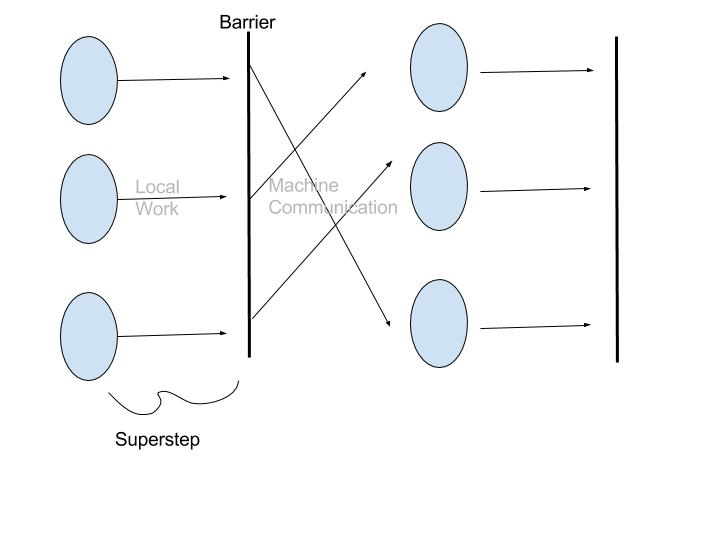
\includegraphics[width=8cm, height=8cm]{590SBSPdiagram.jpg}
\begin{enumerate}
\item Originates from PRAM a theoretic programming model assuming small unit costs of memory transaction (doesn't work in practice)
\item Operates in supersteps where all machines do local work. All machines must wait for the other ones to finish their superstep before crossing the "barrier" to communicate with other machines
\item Barriers aren't ideal (machines sit idly) but there is synchronism without deadlocks and races
\item For graphs, vertices and their edges can be split across machines
\end{enumerate}
\item Message Passing Interface
\begin{enumerate}
\item Broadcast: send messages to all
\item Group communication : send message to some
\item Problems that could arise are
\begin{enumerate}
\item Can easily end up in deadlocks
\item There are chances of communication race happening. This leads to non determinism, ex:
    \begin{verbatim}
    if mpi_self == 0
        mpi_recv:(ANY)
        print result
    else
        mpi_send(self, 0)
    \end{verbatim}
    Each time the program is run, not same value may be printed.
\end{enumerate}
\end{enumerate}
\item Though synchronization with barriers can be slow, BSP model is preferred. We want determinism and no deadlocks. BSP addresses all these problems. Communication cycles are not possible in BSP since all sends happen followed by all receives.
\item When there are many edges associated with one vertex and few edges with all other vertices, then superstep time can be prolonged because of this one vertex. Random selection is better for load balancing.
\end{enumerate}
\end{document}